\section{Marco Teórico}
Este capítulo construye los fundamentos teóricos de la investigación siguiendo una progresión de lo general a lo específico: parte de la naturaleza física del recurso solar y del problema de pronóstico de series de tiempo, recorre la evolución de las técnicas predictivas —desde los modelos estadísticos clásicos hasta las arquitecturas de aprendizaje profundo basadas en atención— y culmina en el tránsito del paradigma de entrenamiento local (\textit{one-site}) al global (\textit{multi-site}), que es el eje conceptual sobre el que se articula la solución propuesta para el problema del arranque en frío.

\subsection{Generación Fotovoltaica y el Recurso Solar}
La generación de energía solar fotovoltaica corresponde al proceso de conversión directa de la radiación solar en electricidad mediante el efecto fotovoltaico. La potencia activa de salida de una planta posee una dependencia estocástica respecto a múltiples variables atmosféricas dinámicas \needcite{física del recurso solar / dependencia de la potencia FV respecto a variables meteorológicas}. La variable con mayor correlación directa es la Irradiancia Horizontal Global (GHI), definida como la cantidad total de radiación de onda corta recibida por una superficie horizontal, que integra las componentes directa y difusa \needcite{definición y componentes de la irradiancia solar (GHI, DNI, DHI)}. De forma secundaria, factores térmicos y atmosféricos como la temperatura ambiente, la humedad relativa, la velocidad del viento y, sobre todo, la nubosidad, modulan la eficiencia de conversión de los paneles \needcite{efecto de la temperatura y la nubosidad en la eficiencia fotovoltaica}. En conjunto, la intermitencia de estas variables produce fluctuaciones severas en la inyección de energía a la red, lo que convierte al pronóstico preciso de generación en un insumo crítico para la operación de los sistemas eléctricos con alta penetración renovable \cite{cen2025}.

\subsection{Series de Tiempo y el Problema de Pronóstico}
Una serie de tiempo se define como un conjunto ordenado de observaciones cuantitativas registradas en intervalos de tiempo regulares \cite{Peixeiro2022}. El pronóstico consiste en analizar estas secuencias históricas para proyectar valores futuros, tarea que se apoya en propiedades estructurales de la señal —tendencia, estacionalidad y autocorrelación— y en supuestos como la estacionariedad \cite{Peixeiro2022}. En el dominio energético, el pronóstico fotovoltaico presenta una estacionalidad múltiple y anidada (ciclo diario e interanual) y una fuerte intermitencia inducida por el clima, lo que ha motivado una progresión metodológica desde los modelos lineales clásicos hacia arquitecturas capaces de capturar dependencias no lineales de largo alcance \cite{Benidis2022}.

\subsection{Modelos Estadísticos Clásicos}
La familia de modelos estadísticos constituye el punto de partida histórico del pronóstico de series de tiempo y opera bajo un paradigma estrictamente \textbf{local}: cada modelo se ajusta a los datos históricos de una única serie, sobre la premisa de disponer de un historial largo e ininterrumpido.

El \textbf{suavizado exponencial} (\textit{exponential smoothing}) proyecta el futuro como un promedio ponderado de las observaciones pasadas, asignando pesos que decaen geométricamente hacia atrás en el tiempo; sus variantes de Holt y Holt-Winters extienden la formulación para capturar explícitamente componentes de tendencia y estacionalidad \cite{Peixeiro2022}. Por su parte, la metodología de Box-Jenkins formaliza los modelos \textbf{autorregresivos de media móvil} (ARMA) y su extensión integrada \textbf{ARIMA}, que combina términos autorregresivos, de media móvil y de diferenciación para modelar series no estacionarias \cite{Peixeiro2022}. Las variantes \textbf{SARIMA} y \textbf{SARIMAX} incorporan, respectivamente, la estacionalidad periódica y la influencia de variables exógenas (como las meteorológicas), lo que las hace teóricamente aplicables al pronóstico solar \cite{Peixeiro2022}.

La limitación fundamental de esta familia es triple: asume relaciones predominantemente lineales entre las variables, exige la satisfacción de supuestos estadísticos estrictos (estacionariedad, homocedasticidad) y, por su naturaleza local, requiere un historial extenso de la propia serie para estimar sus parámetros —condición precisamente ausente en el escenario de arranque en frío.

\subsection{Aprendizaje Automático: Ensambles de Árboles de Decisión}
La incorporación del \textit{Machine Learning} al pronóstico permitió relajar los supuestos de linealidad. Los algoritmos basados en ensambles de árboles de decisión mediante potenciación del gradiente (\textit{gradient boosting}), y en particular \textbf{XGBoost}, construyen de forma aditiva una secuencia de árboles donde cada uno corrige los errores residuales del ensamble previo, capturando interacciones no lineales entre las variables de forma eficiente y regularizada \cite{Chen2016}. En el dominio energético, estos algoritmos han demostrado un desempeño competitivo y una alta interpretabilidad al cuantificar la importancia relativa de cada variable meteorológica \cite{rodriguez2023energy}. No obstante, al ser modelos tabulares que aprenden por particionamiento del espacio de características, carecen de capacidad de extrapolación fuera del rango observado en entrenamiento, lo que degrada severamente su desempeño cuando la serie objetivo carece de historial —nuevamente, el problema del arranque en frío.

\subsection{Aprendizaje Profundo para Series Temporales}
El aprendizaje profundo (\textit{Deep Learning}) introdujo la capacidad de aprender representaciones jerárquicas directamente de los datos, superando la necesidad de ingeniería manual de características. Las redes neuronales recurrentes, y en particular la arquitectura \textbf{Long Short-Term Memory} (LSTM) \cite{Hochreiter1997}, incorporaron compuertas de memoria que permiten retener información de estados pasados y mitigar el desvanecimiento del gradiente, habilitando el modelado de dependencias temporales de corto y mediano plazo. Como alternativa a la recurrencia, las redes convolucionales temporales demostraron que arquitecturas puramente convolucionales pueden igualar o superar a las recurrentes en tareas secuenciales, con la ventaja del procesamiento paralelo \cite{Bai2018}.

Un avance conceptual relevante fue el paso del pronóstico puntual al \textbf{pronóstico probabilístico}. El modelo \textbf{DeepAR} \cite{Salinas2020} estructura una red recurrente autorregresiva que, en lugar de un único valor, estima los parámetros de una distribución de probabilidad futura, permitiendo cuantificar analíticamente la incertidumbre de la predicción —una capacidad esencial para la gestión de riesgo en la operación energética. En paralelo, las arquitecturas de expansión en bases, como \textbf{N-BEATS} \cite{Oreshkin2020}, propusieron bloques de proyección sobre bases funcionales interpretables (tendencia y estacionalidad) que alcanzaron desempeño de estado del arte sin recurrencia. Su sucesor, \textbf{N-HiTS}, refina esta idea mediante interpolación jerárquica y muestreo multi-tasa, lo que reduce drásticamente el costo computacional en horizontes largos y lo posiciona como una contraparte moderna y eficiente frente a los modelos atencionales \cite{Challu2023}. Una revisión sistemática del campo documenta esta transición y consolida al aprendizaje profundo como el paradigma dominante en el pronóstico de series de tiempo a gran escala \cite{Benidis2022}.

\subsection{El Mecanismo de Atención y las Arquitecturas Transformer}
La arquitectura \textbf{Transformer} \cite{Vaswani2017} representó una disrupción en el procesamiento secuencial al eliminar la recurrencia en favor del mecanismo de \textbf{autoatención} (\textit{self-attention}), que pondera dinámicamente la relevancia de cada instante de la secuencia respecto a los demás. Al procesar la secuencia completa en paralelo, los Transformers reducen la pérdida de información a largo plazo y escalan eficientemente en el entrenamiento.

Su adaptación al pronóstico de series de tiempo dio lugar a una familia de arquitecturas especializadas. El \textbf{Informer} \cite{Zhou2021} introdujo la autoatención \textit{ProbSparse}, que reduce la complejidad computacional de cuadrática a logarítmica y habilita el pronóstico de secuencias extremadamente largas que antes desbordaban la memoria. El \textbf{PatchTST} \cite{Nie2022} propuso segmentar la señal en parches (sub-ventanas) antes de aplicar la atención, reteniendo la información semántica a nivel de vecindario temporal. El \textbf{Temporal Fusion Transformer} (TFT) se distingue por su diseño explícitamente multivariado: integra redes de selección de variables y codificadores especializados que procesan de forma diferenciada las covariables estáticas (como la ubicación geográfica de la planta) y las dinámicas (irradiancia y temperatura), además de emitir pronósticos por cuantiles \cite{Lim2021}. Esta capacidad de fusionar información heterogénea de manera asimétrica lo convierte en la arquitectura idónea para la transferencia de conocimiento entre plantas.

La supremacía de los Transformers no está exenta de debate: trabajos posteriores mostraron que modelos lineales simples pueden igualar o superar a arquitecturas atencionales sobre-complejas en ciertos escenarios de pronóstico de largo plazo \cite{Zeng2023}, lo que subraya la necesidad de un \textit{benchmarking} riguroso frente a líneas base sólidas. Más recientemente, los modelos de espacio de estados con selección, como Mamba \cite{Gu2023}, han emergido como una alternativa de complejidad lineal a la atención, delineando la frontera actual de la investigación.

\begin{figure}[hbt!]
  \centering
  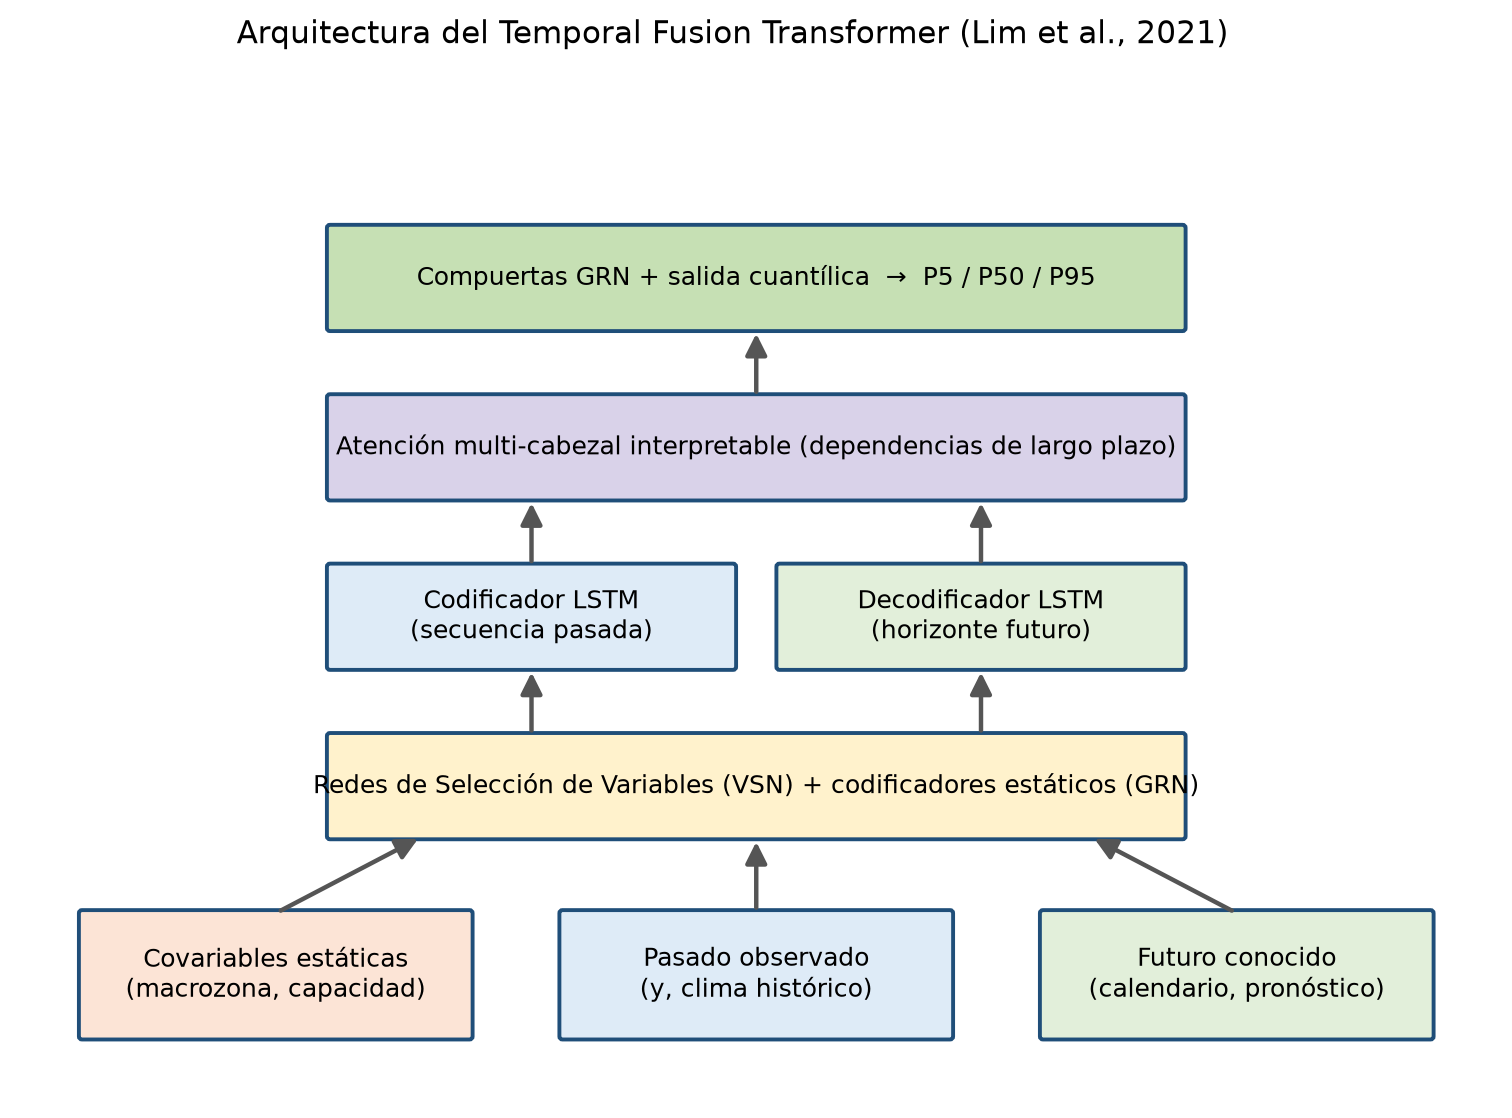
\includegraphics[width=0.82\textwidth]{figuras/fig_tft_arch.png}
  \caption{\label{fig:arquitectura_tft} Arquitectura del Temporal Fusion Transformer, destacando sus compuertas Gated Residual Networks (GRN) y su bloque de atención multipunto.}
\end{figure}

\subsection{Del Paradigma Local al Global: Aprendizaje Multi-Sitio}
Todas las técnicas anteriores pueden desplegarse bajo dos paradigmas de entrenamiento fundamentalmente distintos. En el enfoque \textbf{local} (\textit{one-site}), se ajusta un modelo independiente por cada serie temporal, utilizando exclusivamente su propio historial; es el supuesto operativo tradicional de los modelos estadísticos. En el enfoque \textbf{global} (\textit{multi-site}), un único modelo se entrena de forma simultánea sobre un conjunto de múltiples series, aprendiendo patrones compartidos y regularidades transversales al conjunto \cite{MonteroManso2021}. La evidencia empírica reciente indica que, en conjuntos de series relacionadas y especialmente bajo condiciones de intermitencia o cortes de telemetría, el paradigma global aporta un efecto estabilizador y una mejor generalización que su contraparte local \cite{Damato2026}.

Este paradigma global se materializa a través del \textbf{aprendizaje por transferencia} (\textit{Transfer Learning}), técnica en la que el conocimiento extraído de la resolución de una tarea con abundancia de datos se reutiliza para resolver un problema análogo en un dominio con escasez de datos \cite{PanYang2010}. Aplicado al pronóstico solar, esta concepción adopta la forma de \textbf{aprendizaje multi-sitio} (\textit{Cross-Site Learning}): un modelo de Deep Learning se entrena con la ingesta simultánea de datos de un clúster de plantas fotovoltaicas geográficamente distribuidas y, al correlacionar sus atributos estáticos con las variables dinámicas globales, abstrae el comportamiento atmosférico fundamental subyacente. El modelo resultante puede así emitir pronósticos para una planta nueva reduciendo o eliminando la exigencia de un historial local sustancial.

\begin{figure}[hbt!]
  \centering
  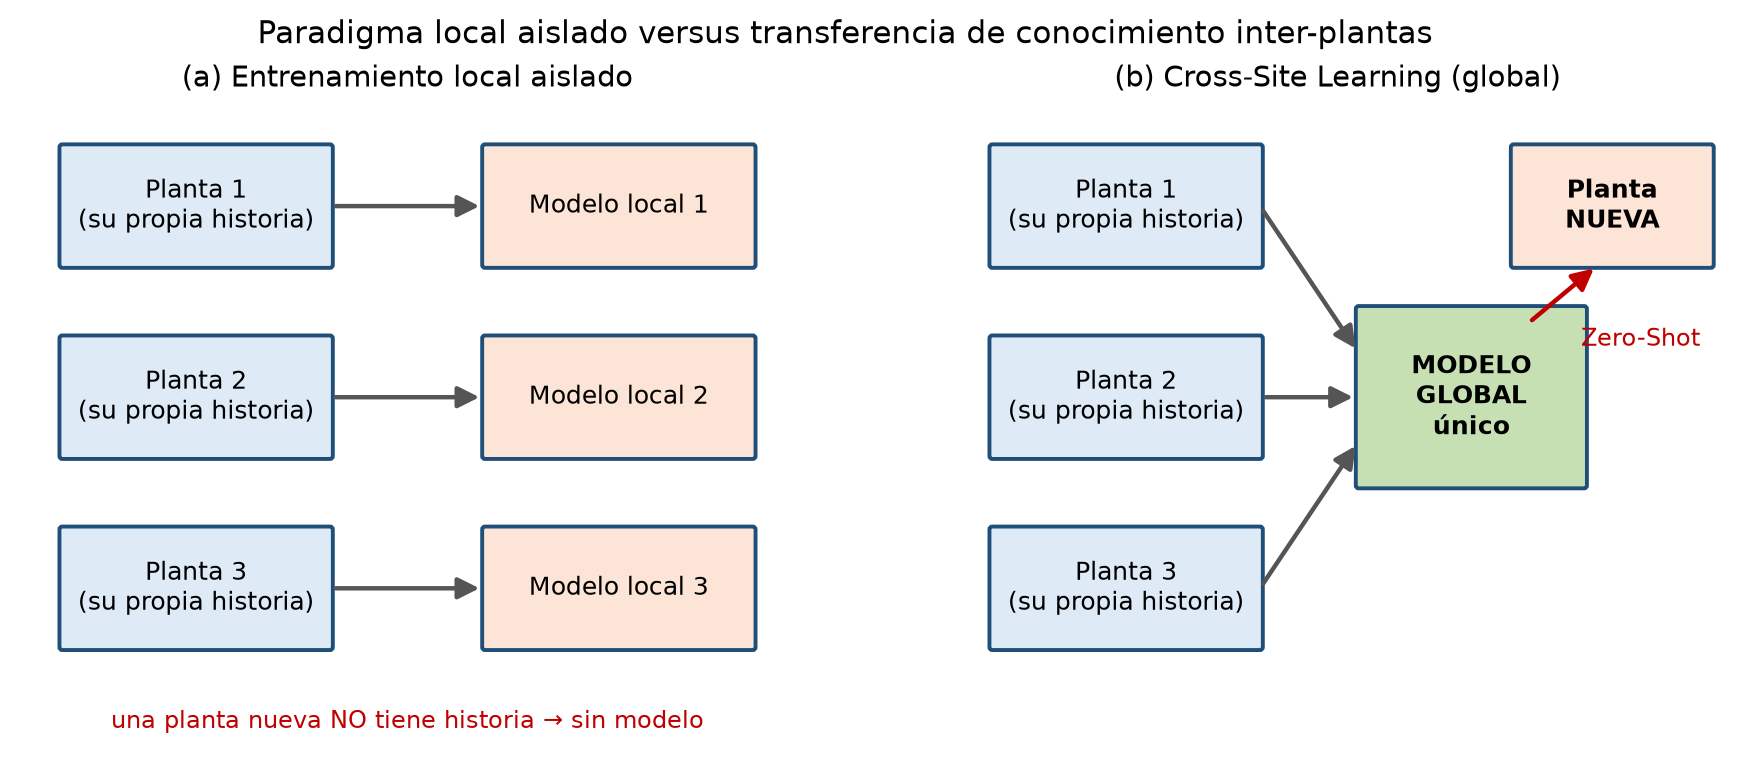
\includegraphics[width=\textwidth]{figuras/fig_cross_site.png}
  \caption{\label{fig:cross_site} Flujo conceptual de transferencia de conocimiento global inter-plantas versus el entrenamiento local y aislado.}
\end{figure}

\subsection{El Problema del Arranque en Frío (Cold-Start)}
El concepto de \textit{Cold-Start} (arranque en frío), originado en los sistemas de recomendación y trasladado al ámbito de las energías renovables, se refiere a la incapacidad de un algoritmo predictivo para generar estimaciones confiables debido a la ausencia parcial o total de datos históricos locales en una instalación recién puesta en marcha \needcite{problema de Cold-Start en pronóstico de energía / sistemas de recomendación}. Dado que los modelos locales —estadísticos, de \textit{Machine Learning} y de \textit{Deep Learning}— requieren extensos registros para modelar la estacionalidad climática anual y evitar el sobreajuste, la fase inicial de operación de un nuevo parque solar se caracteriza por una alta degradación predictiva que impacta la estabilidad de la red de transmisión. El aprendizaje multi-sitio se postula, precisamente, como la vía para transferir el conocimiento climático generalizado de la flota operativa hacia estas instalaciones sin historia.

\subsection{Conclusión acerca de las Herramientas Seleccionadas}
A partir de la revisión precedente queda sustentado el arreglo metodológico del proyecto. Como arquitecturas globales de \textit{Deep Learning} para ejecutar el paradigma \textit{Cross-Site} se seleccionan el \textbf{Temporal Fusion Transformer} (TFT), la arquitectura atencional \textbf{Informer} y la red jerárquica \textbf{N-HiTS}, complementadas por una \textbf{LSTM} global. Como líneas base del paradigma local tradicional se emplean \textbf{XGBoost} y las mismas arquitecturas profundas entrenadas de forma estrictamente aislada por planta. Este contraste —modelos globales frente a modelos locales, sobre un protocolo de evaluación idéntico— provee el marco analítico riguroso necesario para cuantificar empíricamente en qué medida el aprendizaje multi-sitio mitiga el problema del \textit{Cold-Start} bajo escasez informativa extrema.
